\contourlength{1.0pt}

\tikzset{>=latex} % for LaTeX arrow head
\colorlet{myred}{red!85!black}
\colorlet{myblue}{blue!80!black}
\colorlet{mydarkred}{myred!80!black}
\colorlet{mydarkblue}{myblue!60!black}
\tikzstyle{xline}=[myblue,thick]
\def\tick#1#2{\draw[thick] (#1) ++ (#2:0.09) --++ (#2-180:0.18)}
\tikzstyle{myarr}=[myblue!50,-{Latex[length=3,width=2]}]
\def\N{100}

% CONSTANT
\def\xmax{2.2} % max x axis
\def\ymax{1.6} % max y axis




% LINEAR


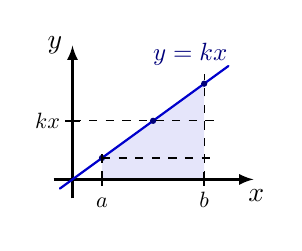
\begin{tikzpicture}
  \message{^^JLinear}
  \def\a{0.17*\xmax}  % first limit
  \def\b{0.76*\xmax}  % last limit
  \def\k{\ymax/\xmax} % slope coefficient
  \fill[myblue!10] (\a,0) -- (\a,\k*\a) -- (\b,\k*\b) |- cycle;
  \draw[->,thick] (0,-0.15*\ymax) -- (0,\ymax+0.1) node[left] {$y$};
  \draw[->,thick] (-0.15*\ymax,0) -- (\xmax+0.1,0) node[right=1,below] {$x$};
  \draw[xline,line cap=round]
    (-0.1*\ymax,-0.1*\k*\ymax) -- (0.9*\xmax,0.9*\k*\xmax)
    node[mydarkblue,above left=-3,scale=0.9] {$y=kx$};
  \fill[mydarkblue]
    (\a,\k*\a) circle(0.04) (\b,\k*\b) circle(0.04)
    ({(\b+\a)/2},{\k*(\b+\a)/2}) circle(0.04);
  \draw[dashed] (\a,0) --++ (0,1.25*\k*\a);
  \draw[dashed] (\b,0) --++ (0,1.10*\k*\b);
  \draw[dashed] (0,{\k*(\b+\a)/2}) --++ (1.1*\b,0);
  \draw[dashed] (\a,\k*\a) --++ ({1.1*(\b-\a)},0);
  \tick{\a,0}{90} node[below=-2,scale=0.8] {\strut$a$};
  \tick{\b,0}{90} node[below=-2,scale=0.8] {\strut$b$};
  \tick{0,{\k*(\b+\a)/2}}{0} node[left=-1,scale=0.8] {$\expval{kx}$};
\end{tikzpicture}
